\chapter{Resultados}
\label{chap:resultados}

\subsection{Análise exploratória}

A partir da coleta de dados realizada pelo POLYMOD, o propósito é elucidar a estruturação das interconexões interpessoais e analisar as implicações decorrentes dessas relações visando uma modelagem em redes. Para isso cada indivíduo foi categorizado em 5 faixas etárias: [0,20) (jovens), [20,30) (jovens adultos), [30,50) (adultos), [50,70) (adultos \textit{seniors}) e maiores de 70 que representam os idosos; a distribuição de cada faixa etária é mostrada na Figura \ref{fig:freq}. Esta categorização reveste-se de relevância considerável, haja vista que a estimação dos parâmetros utilizados é viável com a categorização das idades. 

\begin{figure}[H]
    \centering

    \captionsetup{font=normalsize,skip=0.8pt,singlelinecheck=on,labelsep=endash}
    \caption{Faixas etárias no banco de dados POLYMOD}
    \includegraphics[scale= 0.5]{figuras/faixas_polymod-PIF.png}
        %PIF15102023
    %\captionsetup{font=small}
    \captionsetup{font=small,justification=justified}
    \caption*{Resultados da frequência de cada faixa etária no banco de dados POLYMOD, esse será um dos \textit{inputs} do modelo posteriormente.\\ Fonte: Autor.}

    \label{fig:freq}
\end{figure}

Com base nos dados obtidos, será realizada uma investigação para avaliar a duração, frequência e a presença de contato físico nos encontros em análise. A Figura \ref{fig:graficos} mostra os padrões dos contatos do POLYMOD; é possível ver que quanto mais frequente ou durável é o contato maior a chance dele ter contato físico.
Além disso, quanto mais frequente é o contato maiores as chances da conversa durar mais, por exemplo em contatos diários existe mais de 50\% de chance de que o contato dure mais que 1 hora. Por fim, o gráfico mais recente evidencia que, no ambiente domiciliar, a probabilidade de ocorrência de contato físico é significativamente maior, especialmente em áreas designadas para o lazer. Por contraste, no ambiente profissional, as chances são substancialmente menores, sendo considerado o cenário menos propenso a esse tipo de interação.

\begin{figure}[H]
    \centering
    \captionsetup{font=normalsize,skip=0.8pt,singlelinecheck=on,labelsep=endash}
    \caption{Probabilidade de contato físico}
    \includegraphics[scale= 0.45]{figuras/graficos-PIF.png}
\captionsetup{font=small,justification=justified}
    \caption*{Ilustra a relação entre a frequência e a duração dos contatos com a probabilidade de contato físico, mostrando que contatos mais frequentes e duradouros têm maior probabilidade de envolver contato físico. Além disso, o ambiente domiciliar apresenta maior probabilidade de contato físico, especialmente nas áreas de lazer, em comparação ao ambiente profissional, onde a probabilidade é consideravelmente menor. Todas as correlações são altamente significantes.\\ Fonte: Autor.}
    \label{fig:graficos}
\end{figure}


Um elemento importante que foi investigado foi como as idades influenciam nas conexões entre os indivíduos da rede. Na Figura \ref{fig:contatos_faixa} nota-se como é a distribuição de idades da pesquisa. Ao analisar a distribuição de ligações por faixa etária é percebido que seguem uma distribuição geométrica, que pode ser escrita como $P \propto (1 - p)^xp$ ou $P \propto e^{-\lambda x}(1 - e^\lambda)$. Na Figura \ref{fig:contatos_faixa} temos o estudo das distribuições como se fosse da segunda forma, no eixo das abscissas o grau e no eixo das ordenadas o logaritmo da probabilidade, com isso é encontrado uma reta com Mínimos Quadrados na qual o coeficiente angular é igual ao $\lambda$ e seu respectivo $R^2$. 

\begin{figure}[H]
    \centering
    \captionsetup{font=normalsize,skip=0.8pt,singlelinecheck=on,labelsep=endash}
    \caption{Influência das idades nas conexões}
    \includegraphics[scale= 0.3]{figuras/contatos_faixa.png}
    \captionsetup{font=small,justification=justified}
    \caption*{Ilustra a influência das idades nas 
    conexões da rede social, observando uma distribuição geométrica nas ligações por faixa etária.\\ Fonte: Autor.}
    \label{fig:contatos_faixa}
\end{figure}

A pesquisa também revela a relação entre a faixa etária de um indivíduo que preencheu o questionário e a distribuição de suas ligações. A Figura \ref{fig:heat} ilustra para cada faixa etária das linhas, a frequência relativa de conexões com as faixas etárias das colunas. Notavelmente, a faixa etária 3 apresenta a maior frequência de conexões, sendo composta majoritariamente por indivíduos que estão na fase produtiva da vida, muitas vezes já com família estabelecida. Em contraste, a última faixa etária demonstra a menor frequência de conexões, presumivelmente devido às dificuldades associadas a essa fase da vida.

\begin{figure}[H]
    \centering
    \captionsetup{font=normalsize,skip=0.8pt,singlelinecheck=on,labelsep=endash}
    \caption{Frequência média de conexões por faixa etária}
    \includegraphics[scale= 0.5]{figuras/h-PIF.png}
    \captionsetup{font=small,justification=justified}
    \caption*{Mostra a frequência média de conexões por faixa etária, ressaltando que a faixa etária 3, associada à vida profissional e familiar, possui a maior frequência de conexões, enquanto a última faixa apresenta a menor frequência devido às dificuldades inerentes a essa fase da vida. \\Fonte: Autor}
    \label{fig:heat}
\end{figure}

Por último, a Figura \ref{fig:mediastd} apresenta duas matrizes de calor que ilustram a média e o desvio padrão do tempo de contato entre diferentes faixas etárias. A matriz da média mostra que as faixas etárias tendem a ter maior tempo de contato consigo mesmas e com faixas etárias adjacentes, com tempos decrescentes à medida que a diferença de idade aumenta. Notavelmente, a Faixa Etária 1 possui os maiores tempos médios de contato consigo mesma e com a Faixa Etária 2, enquanto os tempos são menores com as faixas etárias superiores e a Faixa Etária 4 apresenta contato elevado com a Faixa Etária 5.

\begin{figure}[H]
    \centering
    \captionsetup{font=normalsize,skip=0.8pt,singlelinecheck=on,labelsep=endash}
    \caption{Média e desvio-padrão dos tempos de contato entre faixas etárias}
    \includegraphics[scale= 0.32]{figuras/media_std.png}
    \captionsetup{font=small,justification=justified}
    \caption*{A imagem mostra a média e o desvio padrão do tempo de contato entre diferentes faixas etárias. A matriz da média indica que o contato é mais intenso dentro da mesma faixa etária e entre faixas etárias adjacentes, reduzindo conforme aumenta a diferença de idade. A matriz do desvio padrão mostra maior variação nos contatos dentro da mesma faixa e entre adjacentes, com menor variação entre faixas mais distantes. \\Fonte: Autor}
    \label{fig:mediastd}
\end{figure}

A matriz do desvio padrão indica que a variação no tempo de contato é mais significativa dentro da mesma faixa etária e com faixas etárias adjacentes, sugerindo maior inconstância nesses contatos. A Faixa Etária 1 apresenta o maior desvio padrão consigo mesma, seguido por desvios elevados com as Faixas Etárias 2 e 3, e menores com as Faixas Etárias 4 e 5. As Faixas Etárias 2 e 3 também exibem variações notáveis consigo mesmas e com faixas adjacentes, enquanto a Faixa Etária 4 tem maior variação com a Faixa Etária 5.

\subsection{Resultados da Rede gerada}

Os dados das Figuras \ref{fig:contatos_faixa} e \ref{fig:heat} foram utilizados como \textit{inputs} do Modelo de Configuração Ponderado, 

Especificamente, com os dados da Figura~\ref{fig:contatos_faixa} foi obtida a distribuição empírica do grau de cada nó de cada faixa etária e com os dados da Figura~\ref{fig:heat} foram estimados os parâmetros de uma distribuição multinomial para estabelecer quantas ligações vão para cada faixa etária. A partir disso e dado um valor de $p$ (parâmetro que aumenta o coeficiente de agrupamento) foi construída a rede para acontecer a simulação da epidemia. As características dessa rede são mostradas na Figura \ref{fig:regressao}
mostra-se como evolui o agrupamento com o incremento de $p$, que cresce com $C \propto p^{\alpha}$, tanto o agrupamento médio quanto o total no qual $\alpha_{medio } = 0.46$ e $\alpha_{total } = 0.55$. Após a aplicação do algoritmo foi recolhido os dados da rede e observou-se que para qualquer valor de $p$ a distribuição de graus tinha a mesma distribuição que a encontrada pela Figura \ref{fig:contatos_faixa} a partir do teste de Kolmogorov-Smirnov (Figura \ref{fig:comparacao}) \cite{manual}. Na Figura \ref{fig:modelo}
mostra-se a diferença absoluta ao final do algoritmo da proporção de conexões de cada faixa etária em comparação com a Figura \ref{fig:heat}, tendo uma diferença maior entre as conexões com faixa etária 1. Além disso na Figura \ref{fig:correlation} apresenta a correlação linear entre o Agrupamento e o Grau com o incremento de $p$, nele é possível notar que o valor decresce, ou seja nós com maior grau tendem a ter menos agrupamento, isso acontece, provavelmente, porque com grau muito alto existem muito mais combinações entre os sítios e o algoritmo não consegue contemplar esses nós com alto grau, expondo uma limitação do algoritmo.
\begin{figure}[H]
    \centering
    %PIF27092023
    \captionsetup{font=normalsize,skip=0.8pt,singlelinecheck=on,labelsep=endash}
    \caption{Agrupamento da rede em função de $p$}
    %PIF27092023 É possível apagar o enquadramento branco?        
    %\includegraphics[scale= 0.5]{figuras/clustering_vs_p.png}
    \includegraphics[scale= 0.45]{figuras/clustering_vs_p.png}
    \captionsetup{font=small,justification=justified}    \caption*{Evolução do agrupamento da rede em função 
    do incremento do valor de $p$, foi utilizada uma regressão linear para saber qual a função que rege encontrando $C \propto p^{\alpha}$.\\Fonte: Autor}
    \label{fig:regressao}
\end{figure}

\begin{figure}[H]
    \centering
    
    \captionsetup{font=normalsize,skip=0.8pt,singlelinecheck=on,labelsep=endash}
    \caption{Resultados da proporção de conexões entre faixas}
    \includegraphics[scale= 0.4]{figuras/modelo.png}
    \captionsetup{font=small,justification=justified}
    \caption*{ A figura mostra a diferença absoluta entre a matriz de proporções de conexões entre as faixas etárias do modelo e do encontrado no POLYMOD essa diferença se mantém constante independe do valor de $p$.}
    \label{fig:modelo}
\end{figure}
\begin{figure}[H]
    \centering
    \captionsetup{font=normalsize,skip=0.8pt,singlelinecheck=on,labelsep=endash}
    \caption{Distribuição de Graus $p = 1.0$}
    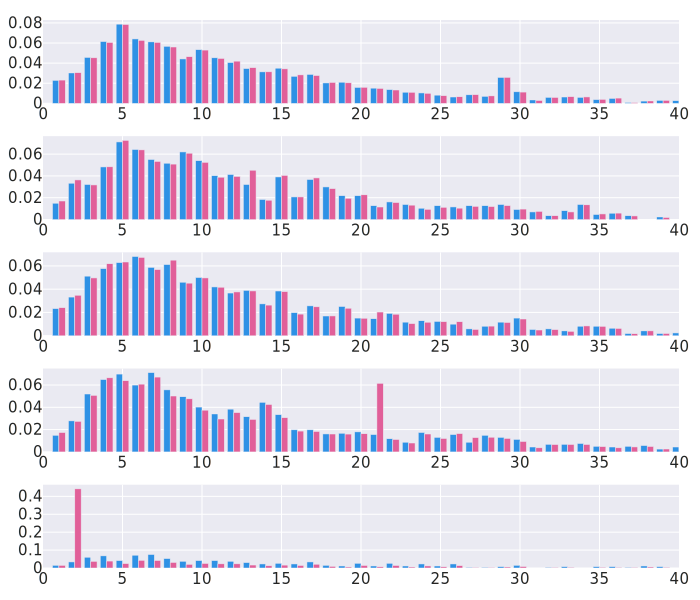
\includegraphics[scale= 0.4]{figuras/comparacao.png}
    \captionsetup{font=small,justification=justified}
    \caption*{Comparação de como fica a distribuição de graus comparando modelo com $p = 1.0$ com dados do POLYMOD, é possível ver todas as faixas foram bem no teste de comparação.\\Fonte: Autor}
    \label{fig:comparacao}
\end{figure}

\begin{figure}[H]
    \centering
    \captionsetup{font=normalsize,skip=0.8pt,singlelinecheck=on,labelsep=endash}
    \caption{Agrupamento da rede em função de $p$}
    \includegraphics[scale= 0.45]{figuras/correlation.png}
    \captionsetup{font=small,justification=justified}    \caption*{Evolução do agrupamento da rede em função 
    do incremento do valor de $p$, foi utilizada uma regressão linear para saber qual a função que rege encontrando $C \propto p^{\alpha}$.\\Fonte: Autor}
    \label{fig:correlation}
\end{figure}

\subsection{Resultados do Modelo de Infecção}

Em suma o modelo utilizado é o Modelo de Configuração Ponderado usando como entrada uma distribuição de graus empírica, a distribuição de faixas etárias brasileira e a distribuição de ligações entre faixas etárias encontradas no banco de dados do POLYMOD, no caso da infecção os parâmetros são os que foram encontrados na literatura ou calculados pelo OpenDataSUS, além disso com o POLYMOD foram calculados as médias e desvios do tempo de contato entre os indivíduos que serão considerados. A simulação acontece do dia 0 até o dia 465 iniciando com 10 nós infectados — para garantir que a simulação não termine cedo — no compartimento Exposto e todos os outros sítios como Suscetíveis. A vacinação ocorre no dia 100, nesse dia são aplicadas vacinas para uma fração $f$ da rede para sítios no compartimento Suscetível,Exposto , Recuperado ou Assintomático dado um critério de prioridade que é determinado pelo valor das centralidades introduzidas anteriormente. Se o indivíduo não estiver apto a ser vacinado no dia e após todos os aptos serem vacinados ainda existirem vacinas sobrando, então se ele atingir um dos compartimentos aptos ele será vacinado.

Para as centralidades que dependem da ponderação nos nós foram utilizadas a probabilidade do nó ser assintomático e a probabilidade dele morrer, para centralidades que originalmente não utilizam ponderação dos nós, apenas nas arestas utilizamos a seguinte mudança:
\begin{equation}
    Z_{\nu,\mu} = w_{\nu,\mu}\cdot(\Theta_\nu + \Theta_\mu).
\end{equation}
O valor de $\Theta_\nu$ e $\Theta_\mu$ e das centralidades com ponderação dos nós será feito de duas abordagens diferentes: Altruísta e a Individualista. A Altruísta será calculando as centralidade pensando que o nó $\nu$ a ser calculado esteja tentando infectar as outras pessoas na rede e matar elas, na abordagem Individualista as centralidades são calculadas pensando no nó $\nu$ sendo infectado por todas as outras pessoas na rede e morrer.

Após a implementação do modelo epidemiológico no modelo de redes escolhidos foram escolhidos pela performasse do algoritmo que após o dia 100 a infecção estabilizava e esse seria o dia da vacinação, deste modo simula-se a situação real na qual a vacina só se tornou disponível após a COVID-19 já ter se espalhado por todo o mundo. Anteriormente a esse dia a rede se comporta, para $p = 0$ (com agrupamento médio de 0.01), de acordo com as Figuras \ref{fig:pre_vacina} e \ref{fig:pre_vacina_mortos}. A Figura \ref{fig:pre_vacina} mostra a evolução da epidemia, em que pode-se observar que a proporção de indivíduos suscetíveis diminui rapidamente até o dia 25, que é o tempo de incubação, para posteriormente aumentar e atingir um estado de estabilidade. A fração de indivíduos infectados (a soma da fração de assintomáticos com a de sintomáticos) aumenta até atingir um pico, com  30\% da população total sendo infectada simultaneamente, seguido por um declínio. Finalmente, a fração de indivíduos recuperados aumenta até que 58\% da população esteja nesse estado, estabilizando posteriormente. Já a Figura \ref{fig:pre_vacina_mortos} mostra a evolução  da  fração de mortos e a fração de hospitalizados, nesse sentido observa-se que o número máximo de hospitalizados observado foi cerca de 0.46\% da rede, enquanto o número de mortos cresce indefinidamente. Neste trabalho, não consideramos a capacidade do sistema hospitalar, pois neste caso, precisaríamos de informações sobre a taxa de recuperação e de morte de sintomáticos que precisariam ser internados e não foram por falta de leitos que não são facilmente determinadas.   

\begin{figure}[H]
    \centering
    \captionsetup{font=normalsize,skip=0.8pt,singlelinecheck=on,labelsep=endash}
    \caption{Fração de Suscetíveis, Infectados e Recuperados antes da aplicação de qualquer estratégia de vacinação}
    \includegraphics[scale= 0.5]{figuras/pre_vacina_nponderado.png}
    \captionsetup{font=small,justification=justified}
    \caption*{Resultados antes da aplicação de qualquer 
    estratégia de vacinação para uma rede $N$ = 10000 com $p $ = 0 após 400 realizações. Inicialmente, a proporção de suscetíveis diminui rapidamente, seguida por um aumento e estabilização. A fração de infectados atinge um pico, afetando 
    40\% da população, e depois diminui. Paralelamente, a proporção de recuperados aumenta e estabiliza em 71\% da população.}
    \label{fig:pre_vacina}
\end{figure}

\begin{figure}[H]
    \centering
    \captionsetup{font=normalsize,skip=0.8pt,singlelinecheck=on,labelsep=endash}
    \caption{Fração de Hospitalizados e Mortos antes da aplicação de qualquer estratégia de vacinação}
    \includegraphics[scale= 0.5]{figuras/pre_vacina_mortos_nponderado.png}
    %\includegraphics[scale= 0.4]{figuras/pre_vacina_mortos-PIF.png}
    \captionsetup{font=small,justification=justified}
    \caption*{Simulações foram feitas para uma rede $N$ = 10000 com $p $ = 0 após 400 realizações. O gráfico mostra que a Fração de Hospitalizados chega a um limite máximo de pessoas que podem estar no estágio ao mesmo tempo enquanto que a fração de mortos cresce indefinidamente até chegar em aproximadamente 0.6\% da rede.}
    \label{fig:pre_vacina_mortos}
\end{figure}

Com o aumento de $p$ surgem diferenças com o comportamento da infecção, a Figura mostra \ref{fig:pre_vacina_mortos_p} que a rede tem uma quantidade menor de mortos, contudo a infecção demora mais para crescer, decair e estabilizar, ou seja o agente permanece mais tempo na rede, isso se deve, provavelmente, ao fato de que em média os idosos tem conexões menores e sabemos anteriormente que o MCP aumenta o agrupamento de nós com poucas conexões e que os mais idosos tem mais conexões com os mais novos pois precisam de cuidados e esses têm pouca chance de morrer mas tem mais conexões, portanto o que deve acontecer é que a infecção se espalha mais no grupo dos mais jovens.

%LCR10072024: É possível exibir gráficos com o número de mortos por faixa etária? E também exibir gráficos com o número de infectados por faixa etária?

\begin{figure}[H]
    \centering
    \captionsetup{font=normalsize,skip=0.8pt,singlelinecheck=on,labelsep=endash}
    \caption{Fração de Mortos e Hospitalizados antes da aplicação de qualquer estratégia de vacinação para diferentes valores de $p$}
    \vspace{5pt}
    \includegraphics[width=\textwidth]{figuras/pre_vacina_mortos_p_nponderado.png}
    \captionsetup{font=small,justification=justified}
    \caption*{Resultados para fração de Mortos e Hospitalizados e função do tempo antes da aplicação de qualquer estratégia de vacinação para uma rede $N$ = 10000 para diferentes valores de $p$. Quanto maior o $p$ menor a fração de mortos e o número de Expostos tende a demorar a estabilizar, resultado das conexões entre faixas.}
    \label{fig:pre_vacina_mortos_p}
\end{figure}

Para finalizar, fizemos a comparação entre como a rede se espalha nos primeiros 100 dias no caso ponderado e não ponderado nesse caso  não houve uma diferença significativa entre o avanço da infecção, a Figura \ref{fig:compara_ponderado_nponderado} mostra para Expostos que a diferença é pouco perceptível isso é visível para qualquer compartimento da rede. Apesar disso será feita a análise das centralidades comparando caso ponderado e não ponderado, porém no caso da infecção pré-vacina não há diferença o que acarreta numa simplificação do modelo o que favorece o tempo computacional dos algoritmos.

\begin{figure}[H]
    \centering
    \captionsetup{font=normalsize,skip=0.8pt,singlelinecheck=on,labelsep=endash}
    \caption{Fração de Infectados com diferentes estratégias de vacinação e $p$ = 0.0}
    \includegraphics[scale= 0.5]{figuras/compara_ponderado_nponderado.png}
    \captionsetup{font=small,justification=justified}
    
    \caption*{ Após 60 dias, diferentes estratégias de vacinação foram aplicadas, mostrando variação no número de infectados. As estratégias de priorização de graus e centralidade de intermediação foram mais eficazes em conter a proliferação, enquanto as estratégias baseadas em idade e aleatória foram as menos eficazes, apresentando desempenho quase equivalente. As demais estratégias, com exceção da centralidade excêntrica, mostraram comportamento semelhante.}
    \label{fig:compara_ponderado_nponderado}
\end{figure}

Após os 100 dias, foi aplicado a vacina com diversas estratégias seguindo as centralidades em redes apresentadas anteriormente. Ao final foram coletadas o tempo total hospitalizado $T_H$, a fração de mortos $F_M$ e fração de indivíduos necessária para extinguir a doença $F_I$. Assim para cada parâmetro foi feito um \textit{ranking} mostrando para as melhores centralidades, para $T_H$ e $F_M$ foi integrado a área do gráfico de parâmetro \textit{versus} $f$. Para determinar qual centralidade apresentou o melhor desempenho geral, calculou-se a média dos respectivos valores de cada centralidade para cada parâmetro avaliado. A qualidade de cada centralidade é varia perante a rede, ou seja, com a alteração de $p$ o \textit{ranking} será diferente e poderá existir diferentes melhores estratégias, seria então necessário estimar os valores de $p$ da rede real para saber qual seria a melhor estratégia. 

A Figura \ref{fig:resultados_metricas} para o caso sem ponderação compara como ficaram os resultados para $p = 0$ e $p = 1$ mostrando 4 métricas, o caso aleatório, idade, a melhor na métrica e a melhor na média, quando o gráfico apresenta apenas 3 curvas significa que a melhor na métrica é a mesma para melhor na média. Esse esquema será repetido na Figura \ref{fig:resultados_metricas_ponderado}, optamos por motivo de muitas centralidades terem sido testadas - 29 para caso não ponderado e 65 para caso não ponderado - para ver os resultados de todas as métricas consulte o Anexo 1.

É possível perceber que em todas as métricas e mudando o valor de $p$ a idade não foi uma boa estratégia no geral contra a doença, um resultado importante é que para extinguir a doença seria necessário vacinar cerca de 80\% da população, entretanto na melhor estratégia foram necessários apenas 32\% para extinguir a doença. Porém é notável que para uma fração menor de 15\% da rede vacinada a idade foi muito boa em comparação às melhores, entretanto ela foi pior para valores maiores. Essa comparação é feita pois foi a principal estratégia utilizada pelos governos.

\begin{figure}[H]
    \centering
    \captionsetup{font=normalsize,skip=0.8pt,singlelinecheck=on,labelsep=endash}
    \caption{Gráfico para cada métrica por fração de vacinados para $p = 0$ e $p = 1.0$ sem ponderação nas arestas}
    \includegraphics[scale= 0.3]{figuras/compara_p_f_nponderado_0.0.png}
    \includegraphics[scale= 0.3]{figuras/compara_p_f_nponderado_1.0.png}
    \captionsetup{font=small,justification=justified}
    
    \caption*{Comparação de cada métrica mostrando se a estratégia fosse aleatória (CR) e se fosse idade (CI) e com as melhores estratégias em cada métrica. Para $p = 0$ a melhor estratégia foi a Utilidade com abordagem Altruísta (A-UT) já no segundo foi a Centralidade de Intermediação (CB). }
    \label{fig:resultados_metricas}
\end{figure}

\begin{figure}[H]
    \centering
    \captionsetup{font=normalsize,skip=0.8pt,singlelinecheck=on,labelsep=endash}
    \caption{Gráfico para cada métrica por fração de vacinados para $p = 0$ e $p = 1.0$ com ponderação nas arestas}
    \includegraphics[scale= 0.3]{figuras/compara_p_f_ponderado_0.0.png}
    \includegraphics[scale= 0.3]{figuras/compara_p_f_ponderado_1.0.png}

    \captionsetup{font=small,justification=justified}
    
    \caption*{ Comparação de cada métrica mostrando se a estratégia fosse aleatória (CR) e se fosse idade (CI) e com as melhores estratégias em cada métrica. Para $p = 0$ a melhor estratégia foi o Page-Rank com pesos nas arestas (WPR) já no segundo foi a Centralidade de Grau (CG). }
    \label{fig:resultados_metricas_ponderado}
\end{figure}

Embora os gráficos forneçam uma indicação preliminar da diferença entre a melhor estratégia em termos de um determinado parâmetro e o desempenho médio, é fundamental realizar uma avaliação para determinar se existe uma diferença significativa entre as métricas, nesse caso foi optado por dado os valores de cada centralidade em cada métrica foi calculado a integral da sua respectiva curva e foi feito a correlação de Spearman entre as métricas. A Figura \ref{fig:Spearman} mostram o valor da correlação para diferentes valores de $p$ para o caso não ponderado e ponderado. É possível ver que as duas métricas mais distintas entre si são $F_M$ e $F_I$ mostrando que a métrica que foca em diminuir a mortalidade uma não necessariamente previne a espalhamento da doença, outrossim com o incremento de $p$ $F_M$ e $T_H$ se tornam mais próximas, por fim existe uma diferença no caso ponderado, na qual as métricas são mais próximas entre si, principalmente a $F_M$ e $T_H$ o que poderia ser descartada nesse caso.

\begin{figure}[H]
    \centering
    \captionsetup{font=normalsize,skip=0.8pt,singlelinecheck=on,labelsep=endash}
    \caption{Correlação entre o ranqueamento entre cada métrica}
    
    \includegraphics[scale= 0.4]{figuras/corr_p.png}
    \\
    \includegraphics[scale= 0.4]{figuras/corr_p_ponderado.png}
    \captionsetup{font=small,justification=justified}
    \caption*{A correlação entre o ranqueamento das métricas mostra que $F_I$ e $F_M$ são as mais diferentes,entretanto com o incremento de $p$ a diferença diminui, para ambos os casos de rede ponderada nas arestas e não ponderada. Além disso na rede ponderada a correlação é muito maior que a não ponderada.}
    \label{fig:Spearman}
\end{figure}

Como mostrado pela Figura \ref{fig:Spearman} as relações entre métricas mudam com o incremento de $p$, assim o próprio \textit{ranking} muda com a variação do parâmetro, assim a Figura \ref{fig:Spearman_p} mostra a correlação de Spearman do \textit{ranking} para cada par de $p$ para rede não ponderada e ponderada, é possível ver que para o caso não ponderado no geral existe uma alta correlação entre os pares, contudo para $F_M$ os valores são menores do que para a $F_I$ e aquele apresenta valores são mais correlacionados com agrupamentos maiores do que este. A conclusão é que no geral o posicionamento das estratégias é bastante estável com o aumento do agrupamento tanto no caso ponderado quanto não ponderado. Isso é bastante útil pois não foi medido o agrupamento da rede real de contatos entre pessoas e com essa estabilidade não se torna tão necessário estimar esse valor.

\begin{figure}[H]
    \centering
    \captionsetup{font=normalsize,skip=0.8pt,singlelinecheck=on,labelsep=endash}
    \caption{Correlação entre o ranqueamento de cada métrica para cada agrupamento}
    
    \includegraphics[scale= 0.4]{figuras/compara_agrupamento_nponderado.png}
    \\
    \includegraphics[scale= 0.4]{figuras/compara_agrupamento_ponderado.png}
    \captionsetup{font=small,justification=justified}
    \caption*{Para cada métrica foi feito uma correlação de Spearman entre os 5 valores de $p$ tanto para ponderação nas arestas quanto sem ponderação. Em ambos os casos mostra-se que a classificação se altera pouco o que é útil pois estimar o agrupamento de uma rede de contatos real é custoso.}
    \label{fig:Spearman_p}
\end{figure}

Anteriormente foram apresentadas as centralidades e as suas versões utilizando ponderamento nas arestas, contudo a utilização da forma ponderada tem um custo computacional bastante considerável, portanto foi avaliado como a métrica foi em comparação com a sua versão ponderada considerando a diferença relativa entre o valor na métrica com ponderação em relação ao valor sem considerar ponderação. A Figura \ref{fig:compara_pesos} mostra como ficou a comparação para dois casos de agrupamento $p = 0$ e pode se perceber que várias métricas não foram bem com o incremento da ponderação nas arestas, principalmente a Utilidade que para $F_I$ teve uma perca de 100\%, mas algumas conseguiram se beneficiar, mas no geral teve um saldo pior.

\begin{figure}[H]
    \centering
    \captionsetup{font=normalsize,skip=0.8pt,singlelinecheck=on,labelsep=endash}
    \caption{Diferença relativa da centralidade com e sem peso nas arestas}
    
    \includegraphics[scale= 0.3]{figuras/compara_pesos_0.0.png}
    \\
    \captionsetup{font=small,justification=justified}
    \caption*{Diferença relativa entre ponderação nas arestas: em todas as métricas a diferença foi irrelevante ou houve uma piora considerável, não utilizá-las reduz o custo computacional do cálculo das centralidades.}
    \label{fig:compara_pesos}
\end{figure}

Diferente da comparação entre o ponderado e não ponderado, a comparação entre Individualista e Altruísta pelo erro relativo é consenso, como mostra a Figura \ref{fig:compara_altruismo}, que o Individualista foi muito pior que a abordagem Altruísta pois ou os valores eram bastante parecidos ou havia uma piora muito grande, no caso da rede ponderada muitas métricas pioraram e nas outras havia pouca mudança já na rede não ponderada houve o contrário.

\begin{figure}[H]
    \centering
    \captionsetup{font=normalsize,skip=0.8pt,singlelinecheck=on,labelsep=endash}
    \caption{Diferença relativa entre abordagem Individualista e Altruista}
    
    \includegraphics[scale= 0.3]{figuras/compara_altruismo_0.0.png}
    \captionsetup{font=small,justification=justified}
    \caption*{Resultado para a diferença relativa entre abordagens: estratégias individualistas foram, em sua maioria, piores que as altruístas. Sem ponderação nas arestas, não houve diferença; com ponderação, houve piora.}
    \label{fig:compara_altruismo}
\end{figure}